\documentclass{beamer}
\usepackage[utf8]{inputenc}

\usetheme{Madrid}
\usecolortheme{default}
\usepackage{amsmath,amssymb,amsfonts,amsthm}
\usepackage{txfonts}
\usepackage{tkz-euclide}
\usepackage{listings}
\usepackage{adjustbox}
\usepackage{array}
\usepackage{tabularx}
\usepackage{gvv}
\usepackage{lmodern}
\usepackage{circuitikz}
\usepackage{tikz}
\usepackage{graphicx}

\setbeamertemplate{page number in head/foot}[totalframenumber]

\usepackage{tcolorbox}
\tcbuselibrary{minted,breakable,xparse,skins}



\definecolor{bg}{gray}{0.95}
\DeclareTCBListing{mintedbox}{O{}m!O{}}{%
  breakable=true,
  listing engine=minted,
  listing only,
  minted language=#2,
  minted style=default,
  minted options={%
    linenos,
    gobble=0,
    breaklines=true,
    breakafter=,,
    fontsize=\small,
    numbersep=8pt,
    #1},
  boxsep=0pt,
  left skip=0pt,
  right skip=0pt,
  left=25pt,
  right=0pt,
  top=3pt,
  bottom=3pt,
  arc=5pt,
  leftrule=0pt,
  rightrule=0pt,
  bottomrule=2pt,
  toprule=2pt,
  colback=bg,
  colframe=orange!70,
  enhanced,
  overlay={%
    \begin{tcbclipinterior}
    \fill[orange!20!white] (frame.south west) rectangle ([xshift=20pt]frame.north west);
    \end{tcbclipinterior}},
  #3,
}
\lstset{
    language=C,
    basicstyle=\ttfamily\small,
    keywordstyle=\color{blue},
    stringstyle=\color{orange},
    commentstyle=\color{green!60!black},
    numbers=left,
    numberstyle=\tiny\color{gray},
    breaklines=true,
    showstringspaces=false,
}
%------------------------------------------------------------
%This block of code defines the information to appear in the
%Title page
\title %optional
{Signal Processing}
\date{March 25,2026}


\author 
{Jnanesh Sathisha karmar - EE25BTECH11029}



\begin{document}



\frame{\titlepage}
\begin{frame}{Question}
\noindent
\textbf{1.2.29} \quad
Consider the discrete-time signal $x(n) = (1/3)^n u(n)$, where $u(n) = 1$ for $n \geq 0$, and define $y(n) = x(-n)$. Then 
\[
\sum_{n=-\infty}^{\infty} y(n)
\]
equals: \hfill (IN 2007)

\vspace{0.5cm}

\noindent
a) $-2/3$ \hspace{2cm}
b) $2/3$ \hspace{2cm}
c) $3/2$ \hspace{2cm}
d) $3$

\end{frame}

\begin{frame}{Theoretical Solution}
\textbf{Method 1}\\
First, let us explicitly write the expression for $y(n)$:
\begin{equation}
y(n) = x(-n) = \left(\frac{1}{3}\right)^{-n} u(-n)
\end{equation}
Because $u(-n) = 1$ only for $n \le 0$, the signal $y(n)$ is zero for all positive values of $n$. We can set up the required summation:
\begin{equation}
S = \sum_{n=-\infty}^{\infty} y(n) = \sum_{n=-\infty}^{0} \left(\frac{1}{3}\right)^{-n}
\end{equation}

To evaluate this, we perform a change of variables. Let $k = -n$. As $n$ goes from $-\infty$ to $0$, $k$ goes from $\infty$ down to $0$.
\begin{equation}
S = \sum_{k=0}^{\infty} \left(\frac{1}{3}\right)^{k}
\end{equation}

\end{frame}

\begin{frame}{Theoretical Solution}
This is a standard infinite geometric series of the form $\sum_{k=0}^{\infty} a r^k = \frac{a}{1 - r}$, where the first term $a = 1$ and the common ratio $r = -\frac{1}{2}$. Since $|r| < 1$, the series converges.
\begin{equation}
S = \frac{1}{1 - \left(\frac{1}{3}\right)} = \frac{1}{1 - \frac{1}{3}} = \frac{1}{\frac{2}{3}} = \frac{3}{2}
\end{equation}
This matches option \textbf{(c)}.
\end{frame}

\begin{frame}{Theoretical Solution}
\section{Method 2: Z-Transform Property (Frequency Domain)}
A more elegant approach utilizes the properties of the Z-transform. The sum of a discrete-time sequence from $-\infty$ to $\infty$ is precisely its Z-transform evaluated at $z = 1$ (which corresponds to the Discrete-Time Fourier Transform evaluated at $\omega = 0$).

\textbf{1. Derivation of the Z-transform of $x(n)$:}

The two-sided Z-transform of a discrete-time signal $x(n)$ is defined fundamentally as:
\begin{equation}
X(z) = \sum_{n=-\infty}^{\infty} x(n) z^{-n}
\end{equation}

Substitute our specific signal $x(n) = \left(\frac{1}{3}\right)^n u(n)$ into the definition. Because the unit step function $u(n) = 0$ for all $n < 0$, the lower limit of our summation changes from $-\infty$ to $0$:
\begin{equation}
X(z) = \sum_{n=0}^{\infty} \left(\frac{1}{3}\right)^n z^{-n}
\end{equation}


\end{frame}


\begin{frame}{Theoretical Solution}
By exponent rules, we can group the terms raised to the power of $n$ together:
\begin{equation}
X(z) = \sum_{n=0}^{\infty} \left(\frac{1}{3} z^{-1}\right)^n
\end{equation}

This is a standard infinite geometric series of the form $\sum_{n=0}^{\infty} r^n$. We know from calculus that this series converges to $\frac{1}{1-r}$ if and only if the absolute value of the common ratio is strictly less than 1 ($|r| < 1$). 

Applying this formula where our common ratio is $r = \frac{1}{3} z^{-1}$:
\begin{equation}
X(z) = \frac{1}{1 - \left(\frac{1}{3} z^{-1}\right)} = \frac{1}{1 - \frac{1}{3}z^{-1}}
\end{equation}

\textbf{Defining the Region of Convergence (ROC):}
The sum only converges (and thus the Z-transform only exists) when $|r| < 1$. Let's solve for $z$:
\begin{equation}
\left| \frac{1}{3} z^{-1} \right| < 1 \implies \frac{1}{3} |z|^{-1} < 1 \implies |z| > \frac{1}{3}
\end{equation}


\end{frame}
\begin{frame}{Theoretical Solution}
Therefore, the Z-transform is $\frac{1}{1 - \frac{1}{3}z^{-1}}$ with an ROC of $|z| > \frac{1}{3}$. This ROC is critical because it tells us that evaluating the function at $z=1$ (which we do in step 3) is mathematically valid, since $1 > 0.33$.

\textbf{2. Time-Reversal Property:}

If $y(n) = x(-n)$, its Z-transform is $Y(z) = X(z^{-1})$.
\begin{equation}
Y(z) = \frac{1}{1 - \frac{1}{3}(z^{-1})^{-1}} = \frac{1}{1 - \frac{1}{3}z}
\end{equation}
The Region of Convergence (ROC) also inverts: $|z^{-1}| > \frac{1}{3} \implies |z| < 3$.

\textbf{3. Evaluate at $z=1$:}

Because $z=1$ lies safely inside the ROC ($1 < 3$), the infinite sum converges to exactly $Y(1)$.
\begin{equation}
\sum_{n=-\infty}^{\infty} y(n) = Y(1) = \frac{1}{1 - \frac{1}{3}(1)} =  \frac{3}{2}
\end{equation}
\end{frame}


\begin{frame}[fragile]
    \frametitle{Python Code}
\begin{lstlisting}[language=Python]
import numpy as np
import matplotlib.pyplot as plt
n = np.arange(-100, 1)
y = (1/3)**(-n)
numerical_sum = np.sum(y)
print(f"Theoretical Sum: 3/2 = {3/2:.5f}")
print(f"Numerical Sum (first 100 terms): {numerical_sum:.5f}")
plt.figure(figsize=(8, 4))
plt.stem(n[-15:], y[-15:], basefmt=" ") 
plt.title('Sequence y(n) approaching 0')
plt.xlabel('n')
plt.ylabel('y(n)')
plt.grid(True)
plt.show()
\end{lstlisting}
\end{frame}


\begin{frame}{Plot-Using only Python}
    \centering
    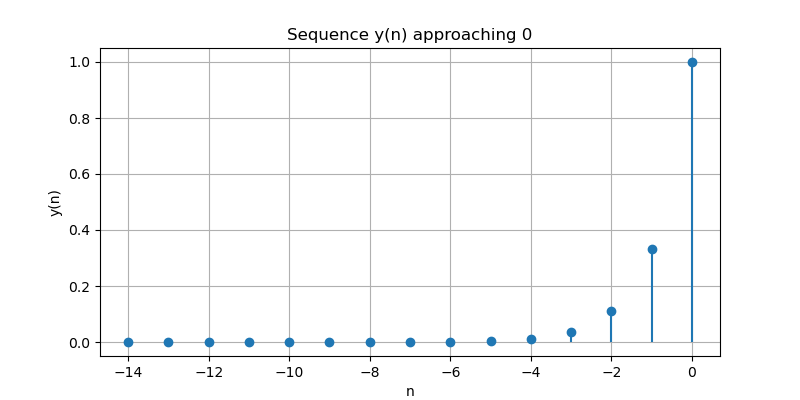
\includegraphics[width=\columnwidth, height=0.8\textheight, keepaspectratio]{question2.png}     
\end{frame}


\begin{figure}
    \centering
    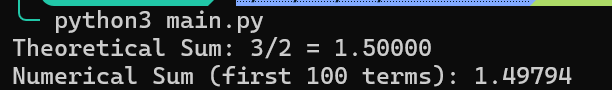
\includegraphics[width=0.9\linewidth]{Screenshot 2026-03-25 161544.png}
    \caption{n=5}
    \label{fig:placeholder}
\end{figure}
\begin{figure}
    \centering
    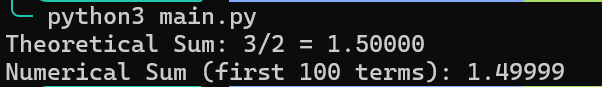
\includegraphics[width=0.9\linewidth]{Screenshot 2026-03-25 161817.png}
    \caption{n=10}
    \label{fig:placeholder}
\end{figure}
\begin{figure}
    \centering
    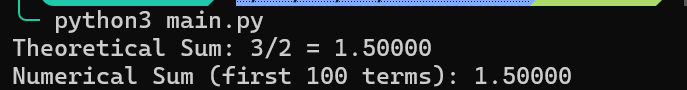
\includegraphics[width=0.9\linewidth]{Screenshot 2026-03-25 161110.png}
    \label{fig:placeholder}
    \caption{n=100}
\end{figure}
\end{document}